\section{Zielsetzung}
In diesem Versuch wird die Biegung elastischer Stäbe untersucht.
Dazu sollen Elastizitätsmodule verschiedener Materialien bestimmt werden. 

\section{Theoretische Grundlage}
Greift eine Kraft an der Oberfläche eines Körpers an und ruft Gestalts- oder Volumenveränderungen an ihm hervor,
wird diese als Spannung bezeichnet.
Die Komponente senkrecht zur Oberfläche wird als Normalspannung $\sigma$ und die parallele Komponente wird als Schubspannung bezeichnet.
Wenn die durch die Spannung hervorgerufene Längenänderung klein genug ist, 
ergibt sich durch das Hookesche Gesetz 

\begin{equation}
\sigma = E \frac{\Delta L}{L}
\end{equation}

\noindent
der lineare Zusammenhang zwischen der Deformation $\frac{\Delta L}{L}$ und der angreifenden Spannung $\sigma$.
Dabei ist der Proportionalitätsfaktor $E$ das materialabhängige konstante  Elastizitätsmodul,
welches durch Messung der Längenänderung bestimmt werden kann.
Durch geringen Kraftaufwand entsteht eine leichte Veränderung des Körpers, die Biegung,
die gemessen werden kann.
Zunächst wird zwischen zwei Arten der Biegung unterschieden.

\subsection{Einseitige Einspannung}
    Wirkt auf einen einseitig eingespannten elastischen stabförmigen Körper eine Gravitationskraft $F$,
    entsteht eine Durchbiegung $D(x)$ nach Abbildung (\ref{fig:eins}).
    
    \begin{figure}
        \centering
           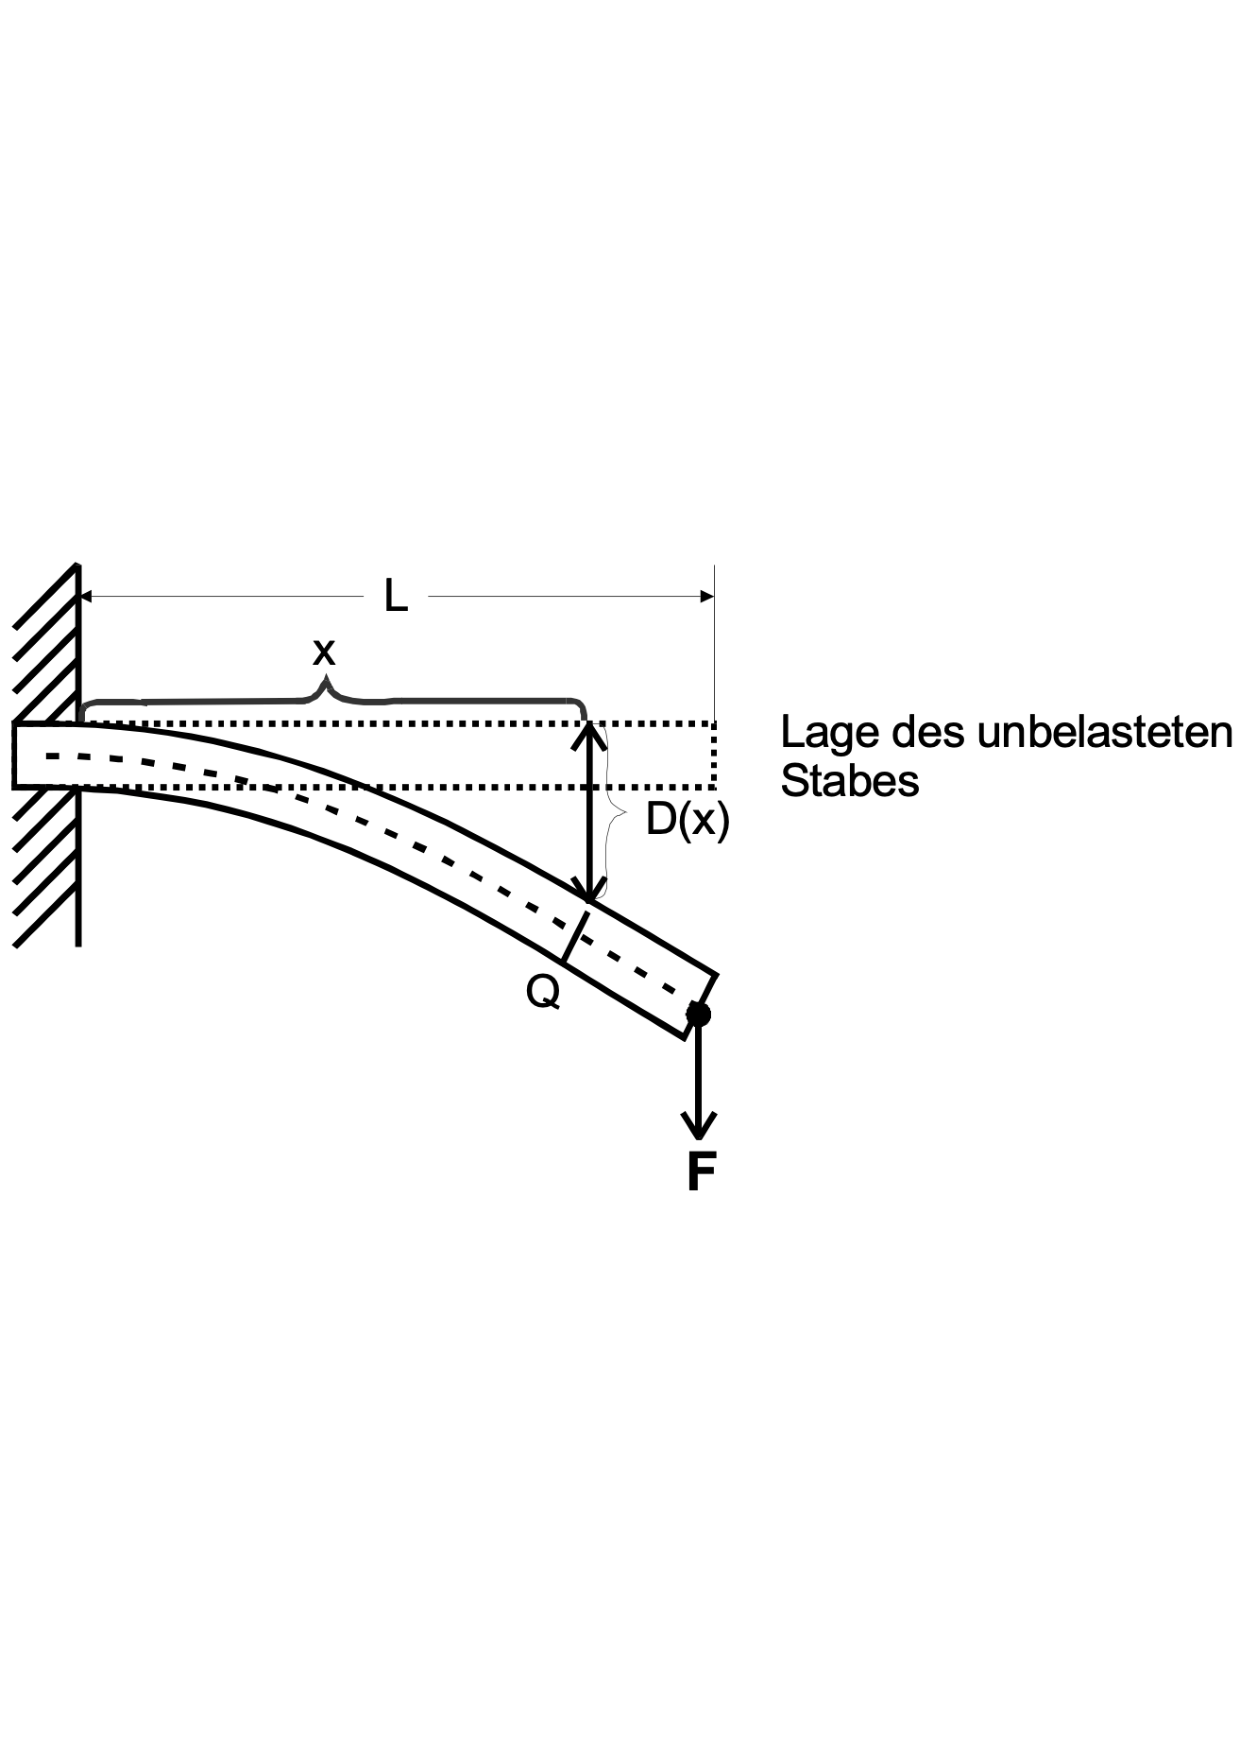
\includegraphics[height=5cm]{eins.pdf}
           \caption{Durchbiegung eines einseitig eingespannten Stabes (Quelle: \cite{V103}).}
           \label{fig:eins}
    \end{figure}
    
    \noindent
    Diese Durchbiegung bewirkt  ein angreifendes Drehmoment

    \begin{equation}
M_F=F \cdot (L-x)
    \end{equation}

    \noindent
    mit der Länge $(L-x)$ des Hebelarms.
    In den oberen Schichten des Stabes treten Zugspannungen und in den unteren Schichten Druckspannungen auf,
    die der Deformation entgegenwirken und ein Drehmoment $M_\sigma$ bewirken,
    welches sich durch die Integration über $Q$ berechnen lässt.
    Es gilt

    \begin{equation*}
M_\sigma = \int_Q y\sigma (y) \, \text{d}q
    \end{equation*}

    \noindent
    mit dem Abstand $y$ des Flächenelementes d$q$ von der neutralen Faser $x$.
    Es ensteht ein Gleichgewichtszustand mit
    
    \begin{equation*}
M_F = M_\sigma
    \end{equation*}

    \noindent
    aus dem sich der Ausdruck 

    \begin{equation}
E\frac{\text{d}^2D}{\text{d}x^2}\int_Q y^2 \, \text{d}q = F(L-x)
    \end{equation}

    \noindent
    mit dem Flächenträgheitsmoment

    \begin{equation}
I := \int_Q y^2 \, \text{d}q(y).
    \end{equation}

    \noindent
    ergibt.
    Nach Integration folgt

    \begin{equation}
D(x) = \frac{F}{2EI} \Bigl(Lx^2-\frac{x^3}{3}\Bigr)
        \label{eqn:deins}
    \end{equation}

    \noindent
    für die Durchbiegung der einseitigen Einspannung.

\subsection{Beidseitige Einspannung}

\begin{figure}
    \centering
       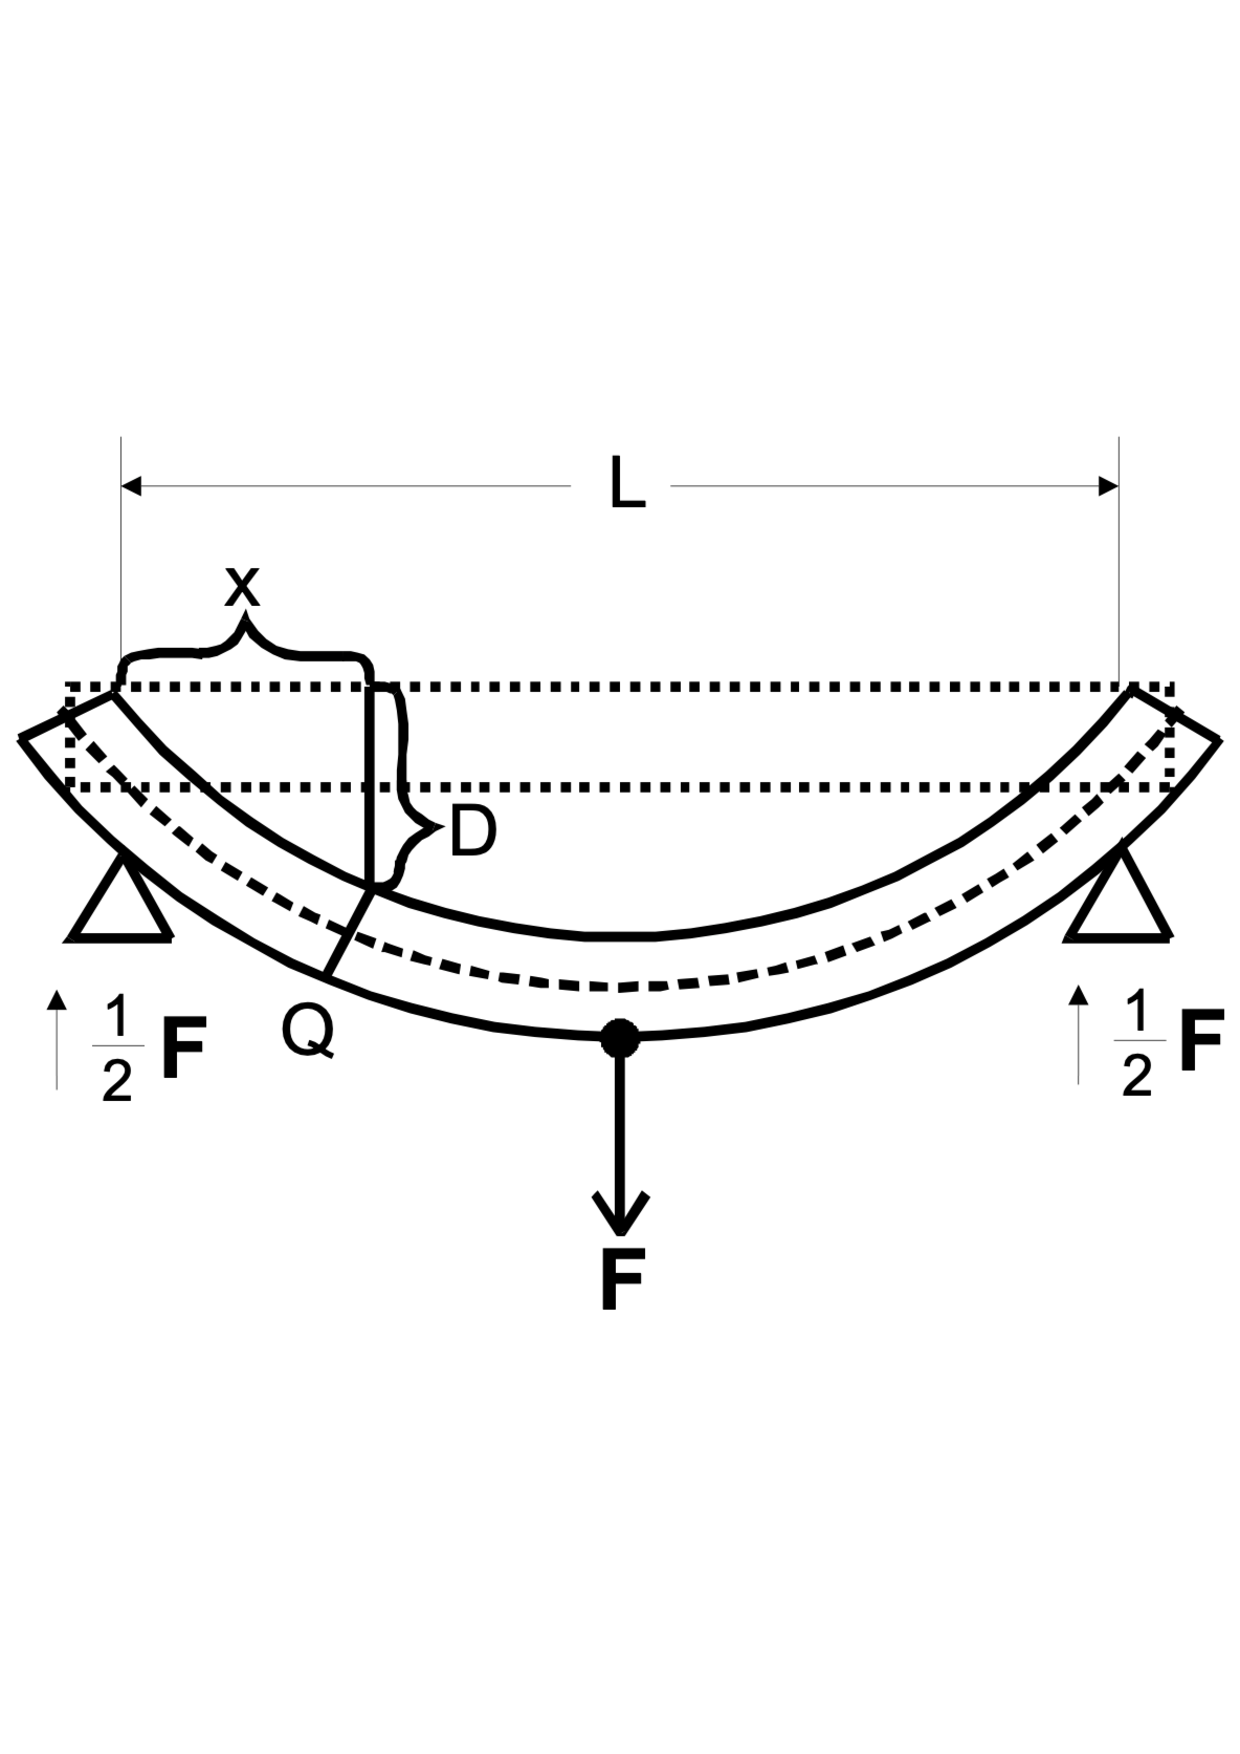
\includegraphics[height=5cm]{beids.pdf}
       \caption{Durchbiegung eines beidseitig eingespannten Stabes (Quelle: \cite{V103}).}
       \label{fig:beids}
\end{figure}

\noindent
Wird der Stab beidseitig aufgelegt, wirkt nach Abbildung (\ref{fig:beids}) die Kraft $F$ in der Mitte 
und der Stab lässt sich in zwei Bereiche mit verschiedenen Drehmomenten unterteilen.
Es gilt












